\section{Message to Prodigal Sons}

\begin{quotex}
O God, thou art my God: early will I seek thee: my soul thirsts for thee. My flesh longs for thee in a dry and thirsty land, where no water is. To see thy power and thy glory, so as I have seen thee in the sanctuary. \flright{\textsc{King David}}

\end{quotex}

We are not writing for the elder son, who stays home playing it safe. As Augustine reminds us, the predestined have what is needed to be saved. The elder son has what he needs; he can ignore us. We write for the \textbf{prodigal son} who gets lost in the world, yet needs a path back. The easy answers no longer have any appeal. The world is offering him less and less, even to the point of transferring his rightful legacy to someone else. In short, is Jack Kerouac or William Buckley your role model?

Jack travelled, wrote about his life, loved, drank, fought in bars, married three times and lived with his mother. Bill had a good dictionary and was born with money and privilege. There is a place for both. Unfortunately, Jack took it too far and was unable to roll it back.

\begin{wrapfigure}{rt}{.25\textwidth}
 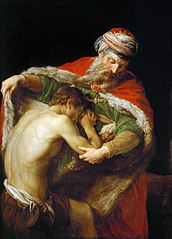
\includegraphics[scale=.5]{a20201202MessagetoProdigalSons-img001.jpg}
\end{wrapfigure} 

In the story, the elder brother stayed home, prayed the rosary in Latin, had 7 children, and knew Denziger by heart. The younger son left in innocence but came back experienced. The father, excited to see his son return, organized a feast and purchased the son's favourite beer. The elder son felt some jealousy, quite unnecessarily. He ensured that the prodigal son had some place to return to, so any resentment is unnecessary.

\paragraph{King David}
David's outer life was ambiguous, full of trials, hardships, triumphs, and blunders. While he was active in the world, he also had a deep spiritual life. The two are not incompatible. Nevertheless, there are those who persist in the notion that a spiritual life needs to follow a pre-ordained pattern and embrace limited modes of thinking. The life of experience is not like that; it is not all sunshine and lollipops.

Actually, in most cases such a life is better, since one learns much more about myself: how to overcome obstacles, face fears, deal with adversity. Yet his relationship to the spiritual world was pure, without illusions, and free from his personal prejudices. His mistakes among the world of men became offerings to God, as revealed in this prayer:

\begin{quotex}
I acknowledge my transgressions and my sin is ever before me. Create in me a clean heart, O God, and renew a right spirit within me. The sacrifices of God are a broken spirit: a broken and a contrite heart, O God, thou will not despise. 

\end{quotex}
\paragraph{The Human State}
Every Tradition agrees that the Human State is unique in the cosmos. A being in this state, unlike those in other states:

\begin{itemize}
\item Experiences both the physical and spiritual world 
\item Knows both good and evil 
\end{itemize}
That is why only such a being can make moral progress.

Rather than focus solely on higher, or even lower, states of being, I've made the decision to describe the Human State in some detail, particularly of this particular being. The predominant impulse in the literature of Tradition has been to leave out everything that reeks of the personal. But is that at all helpful? The journey to higher states cannot be done on a tourist bus.

In the past, children were told that they were brought by a stork. Now, under the influence of a misapplied materiality, we show them anatomically correct renderings of the reproductive system. But isn't the former more correct? Even if the stork version still does not answer the questions surrounding the mystery of birth: ``Who am I? Why am I here?", at least it recognizes a mystery.

The anatomical version doesn't even take the mystery into account or even bother with the question.

\paragraph{Esoteric School}
The Candidate for Initiation must demonstrate fearlessness, freedom from lust and finally loyalty and the ability to be silent. 

There are some who read a little in Tradition, and then go speculating about esoteric schools. Yet they have probably never considered how they would even recognize one; there are no neon signs advertising their presence. Moreover, at least in the West, they may disappear and reappear as conditions change. They are hard to find, but easy to leave.

Many are disappointed with a school because of unrealistic expectations. They may not be willing to face up to their inner nature, once it is revealed to them. A certain type expects to learn metaphysical speculation and leaves when such mere intellectuality is discouraged.

The goal is the primordial state, from which higher states may be reached. Someone recently asked me what the primordial state ``feels" like, as if it could be described in a book. Everyone delights in stories about visiting heaven and in descriptions of higher states of consciousness. But you first need to start where you are, which means, in effect, to ``know thyself."

An esoteric school will start by teaching techniques for self-knowledge and self-observation. There will be training in the three stages of concentration, meditation, and contemplation. The meaning of sacred symbols will be unlocked. It may sometimes be tedious, but over time a true centre is developed. Then other teachings are introduced.

\paragraph{Complicity}
It is necessary to accept responsibility for one's life. In order to understand one's life and integrate the discrete and seemingly random events in life into an awareness of your life as a unified whole, it is necessary to consider the following:

\begin{itemize}
\item Act as though you chose to be born 
\item Act as though you created your life 
\end{itemize}
For an exoteric thinker, those would be points for debate. He would read another book, pore over ancient texts, argue online.

In an esoteric school, the approach is different. First, you would consider these ideas in your Imagination. For one example, imagine this scenario:

Perhaps you are in a bad relationship. How did you contribute to it? What clues about your partner did you ignore or lie about to yourself?

Or imagine that you are choosing your life circumstances before birth. What country, what parents, what religion? Give the imagination free reign to consider what results.

Perhaps over time such exercises will lead to Inspiration or even Intuition.

\paragraph{Overcoming Fear}
Shallow thinkers will tell you to ``follow your bliss", as the key to happiness. So why does not everyone do that? First of all, your bliss cannot be imposed on you from the outside and it fails to acknowledge any obstacles. The path to self-knowledge does not begin with recognizing one's bliss, but, on the contrary, it requires recognizing one's fears. These fears are the hidden parts of oneself and must be exposed to the light, then overcome. See \textit{Qualifications for Initiation}\footnote{\url{https://gornahoor.net/?p=1161}} for descriptions of traditional tests to deal with fears.

\paragraph{The Spiritual Battle}
Don Quixote chose to be a Knight Errant (wandering knight). He ventured out into the world to right wrongs, defend widows and orphans, and earn the love of a beautiful woman.

He found out that the path is hardly easy. If you don't accept consensus reality, they will mock you or call you a ``conspiracy theorist". They will call you ``mad". They will ignore you, deplatform you; your family will ignore you.

\paragraph{Narcissus and Goldmund}
Narcissus creates an intellectual edifice. Everything has its place. All sins and all virtues are accounted for. He then tries to inhabit it. If you try to inhabit it, you are like a hermit crab trying to live in the dead shell of some other animal.

Goldmund goes out into the world and gains experiences. He finds out that It is messy. Goldmund is an artist. That is, while Narcissus is a cataloguer of life, Goldmund is the creator of his life. Ultimately, he gets reconciled with Narcissus.

\paragraph{Better than Tolkien}
People love fantasy stories in worlds populated by unusual beings and wondrous stories. However, our world, the real world if you can experience it in its fullness, is much greater.

You are engaged in spiritual warfare. There are angels and demons using your own mind as the battlefield. You need to overcome obstacles, resist forces from below and respond to influences from above.

The world is hierarchically layered with the planets and stars above, infernal states below. You will encounter Saints, Warriors, Knights, Sages, Mystics, Poets, Artists, Musicians, Philosophers. They will offer clues and advice along the way. Heck, you may even become one yourself.

\paragraph{Lighting up the Chakras}
You can relate to a woman in three ways: sensually, in the heart, or in the head. Those correspond to three different sensations of the I: the I of the body, the I of the heart, the I of the head. If you can relate to her on all three levels, then the three main chakras all light up enabling the free flow of psychic energy. This can be understood on three different levels:

\begin{enumerate}
\item In consciousness: this is the alchemical marriage that leads to the true Self, transcendent to the other thee I's. 
\item With a partner: if your souls can unite, you become a single polar being. This is the most effective, although rare. 
\item Spiritually: you achieve union with God.
\end{enumerate}
\paragraph{Spiritual Infatuation}
You have seen a beautiful woman. You gaze at her, you think about her, you fantasize about her, you desire her; she dominates your consciousness. If you are fortunate enough to meet her, you do anything for her. You notice her clothes, her scent, the smell of her hair after a shower, the way she moves, her smile. When she fully reveals herself, you experience desire in a way you never had previously, you nearly faint from her touch. When she moans or cries out, her pleasure becomes your pleasure. Afterwards, you promise to please her and look for ways to do so. Her joy is a joy to you. Yet, there is more – life is not a series of stepping stones from one pleasure to the next. Her pain becomes your pain, and you vow to alleviate hers.

Do you feel the same way about God? Do you think about Him all day long, do you long to be with Him? Do you try to please him? Like David, do you acknowledge your faults and pray for forgiveness?

\paragraph{The Biography of Jesus}
He received no Nobel prizes. He did not propose an economic program. He did not reveal the laws of physics. He did not teach better living through chemistry. Although he effected cures, he did not eliminate disease itself. He did not write great literature, but relied instead on those who followed. He did not bring peace but rather a sword.

Unlike the rich and famous, his biography as a man, as described the Apostle's Creed, is simple and straight-forward:

He was conceived, he was born, he lived, suffered, died, and was buried. Can't you at least achieve that?

His one superpower was the ability to forgive sins. It is too easy to gloss over that and not understand the magnitude.



\flrightit{Posted on 2020-12-02 by Cologero }

\begin{center}* * *\end{center}

\begin{footnotesize}\begin{sffamily}



\texttt{Ilo Stabet on 2022-04-04 at 09:13 said: }

I wonder if the last section was inspired by Fernando Pessoa, who has a famous poem (famous, at least, for the Portuguese) that ends with: «More than this is Christ/who knew nothing of finances/and didn't seem to have a library».


\end{sffamily}\end{footnotesize}
